\section{Simulation and Theoretical Results}
\label{sec5}
In this section, we compare the bounds obtained via our novel method to bounds obtained using the transfer function method as well as the simulation results for the $5/7,~37/21$ and $23/35$ RSC codes, each with a frame size $N=64$. 
%For each RSC code and a frame size of $N=64$, the codeword is BPSK modulated and transmitted over the AWGN channel. At the receiver end, the Viterbi algorithm is used to decode before a decision is made on the decoded sequence.

We set $d_{\text{max}}=d_{\text{min}}+3$ and using our novel method outlined in the previous section,  we obtained the low-weight codeword component patterns for each RSC code and the results are shown in Tables \ref{novelTab13},  \ref{novelTab14} and \ref{novelTab15} respectively. We then calculate the lower bounds for our novel method and the transfer function using \eqref{novelEq7} and its original version in \cite{ref4} respectively. 
%It is worth noting that in all the tables, the codeword components are arranged in ascending order of codeword weight, with the $d_{\text{free}}$ components at the top of the table.  
%(quarantine)%For each RSC codeThese were obtained by dividing the general form of $h(x)$ for $w_H(\bh)=2$ and ($w_H(\bh)=2$ if it exists) by $f(x)$ and multiplying it by $g(x)$ to obtain $b(x)$ for a given RSC code. This process is repeated doing the same for the general form of $b(x)$. In both cases $a(x),~b(x)$ and $h(x)$ are only added to the list if $w_H(\bc) \leq d_{\text{max}}$.
\begin{table}[htbp]
 \caption{Partial Codeword Component Pattern Distance Spectrum for the $5/7$ RSC code, $d_{\text{free}}=5$}
\centering
 \begin{tabularx}{0.75\textwidth}{Xlll} 
 \hline
 $w_H(c(x))$& $a(x)$ & $b(x)$ & $h(x)$ \\ %[0.5ex] 
 \hline\hline
5&$1$ & $1+x+x^{2}$ & $1+x^2$\\
\hline\hline
6&$1+x^2$ & $1+x+x^3+x^4$ & $1+x^{4}$\\
%\hline
&$1+x$ & $1+x^3$ & $1+x+x^2+x^3$\\
\hline\hline
&$1+x^2+x^4$ & $1+x+x^3+x^5+x^6$ & $1+x^{6}$\\
%\hline\hline
7&$1+x^2+x^3$ & $1+x+x^5$ & $1+x^3+x^4+x^5$\\
%\hline
&$1+x+x^2$ & $1+x^2+x^4$ & $1+x+x^3+x^4$\\
%\hline
&$1+x+x^3$ & $1+x^4+x^5$ & $1+x+x^2+x^5$\\
\hline \hline
8&$1+x^2+x^4+x^6$ & $1+x+x^3+x^5+x^7+x^8$ & $1+x^8$\\
%\hline
&$1+x+x^3+x^4$ & $1+x^6$ & $1+x+x^2+x^4+x^5+x^6$\\
\hline
%======extra
%\hline
%$1+x+x^3+x^5$ & $1+x^4+x^6+x^7$ & $1+x+x^2+x^7$\\
%\hline
%$1+x+x^2+x^4$ & $1+x^2+x^5+x^6$ & $1+x+x^3+x^6$\\
%\hline
%$1+x+x^2+x^3$ & $1+x^2+x^3+x^5$ & $1+x+x^4+x^5$\\
%\hline
%$1+x^2+x^3+x^5$ & $1+x+x^6+x^7$ & $1+x^3+x^4+x^7$\\
%\hline
%$1+x^2+x^3+x^4$ & $1+x+x^4+x^6$ & $1+x^3+x^5+x^6$\\
%\hline
%$1+x^2+x^4+x^5$ & $1+x+x^3+x^7$ & $1+x^5+x^6+x^7$\\
 \end{tabularx}
 
 \label{novelTab13}
\end{table}

\begin{figure}[htbp]
\centering
		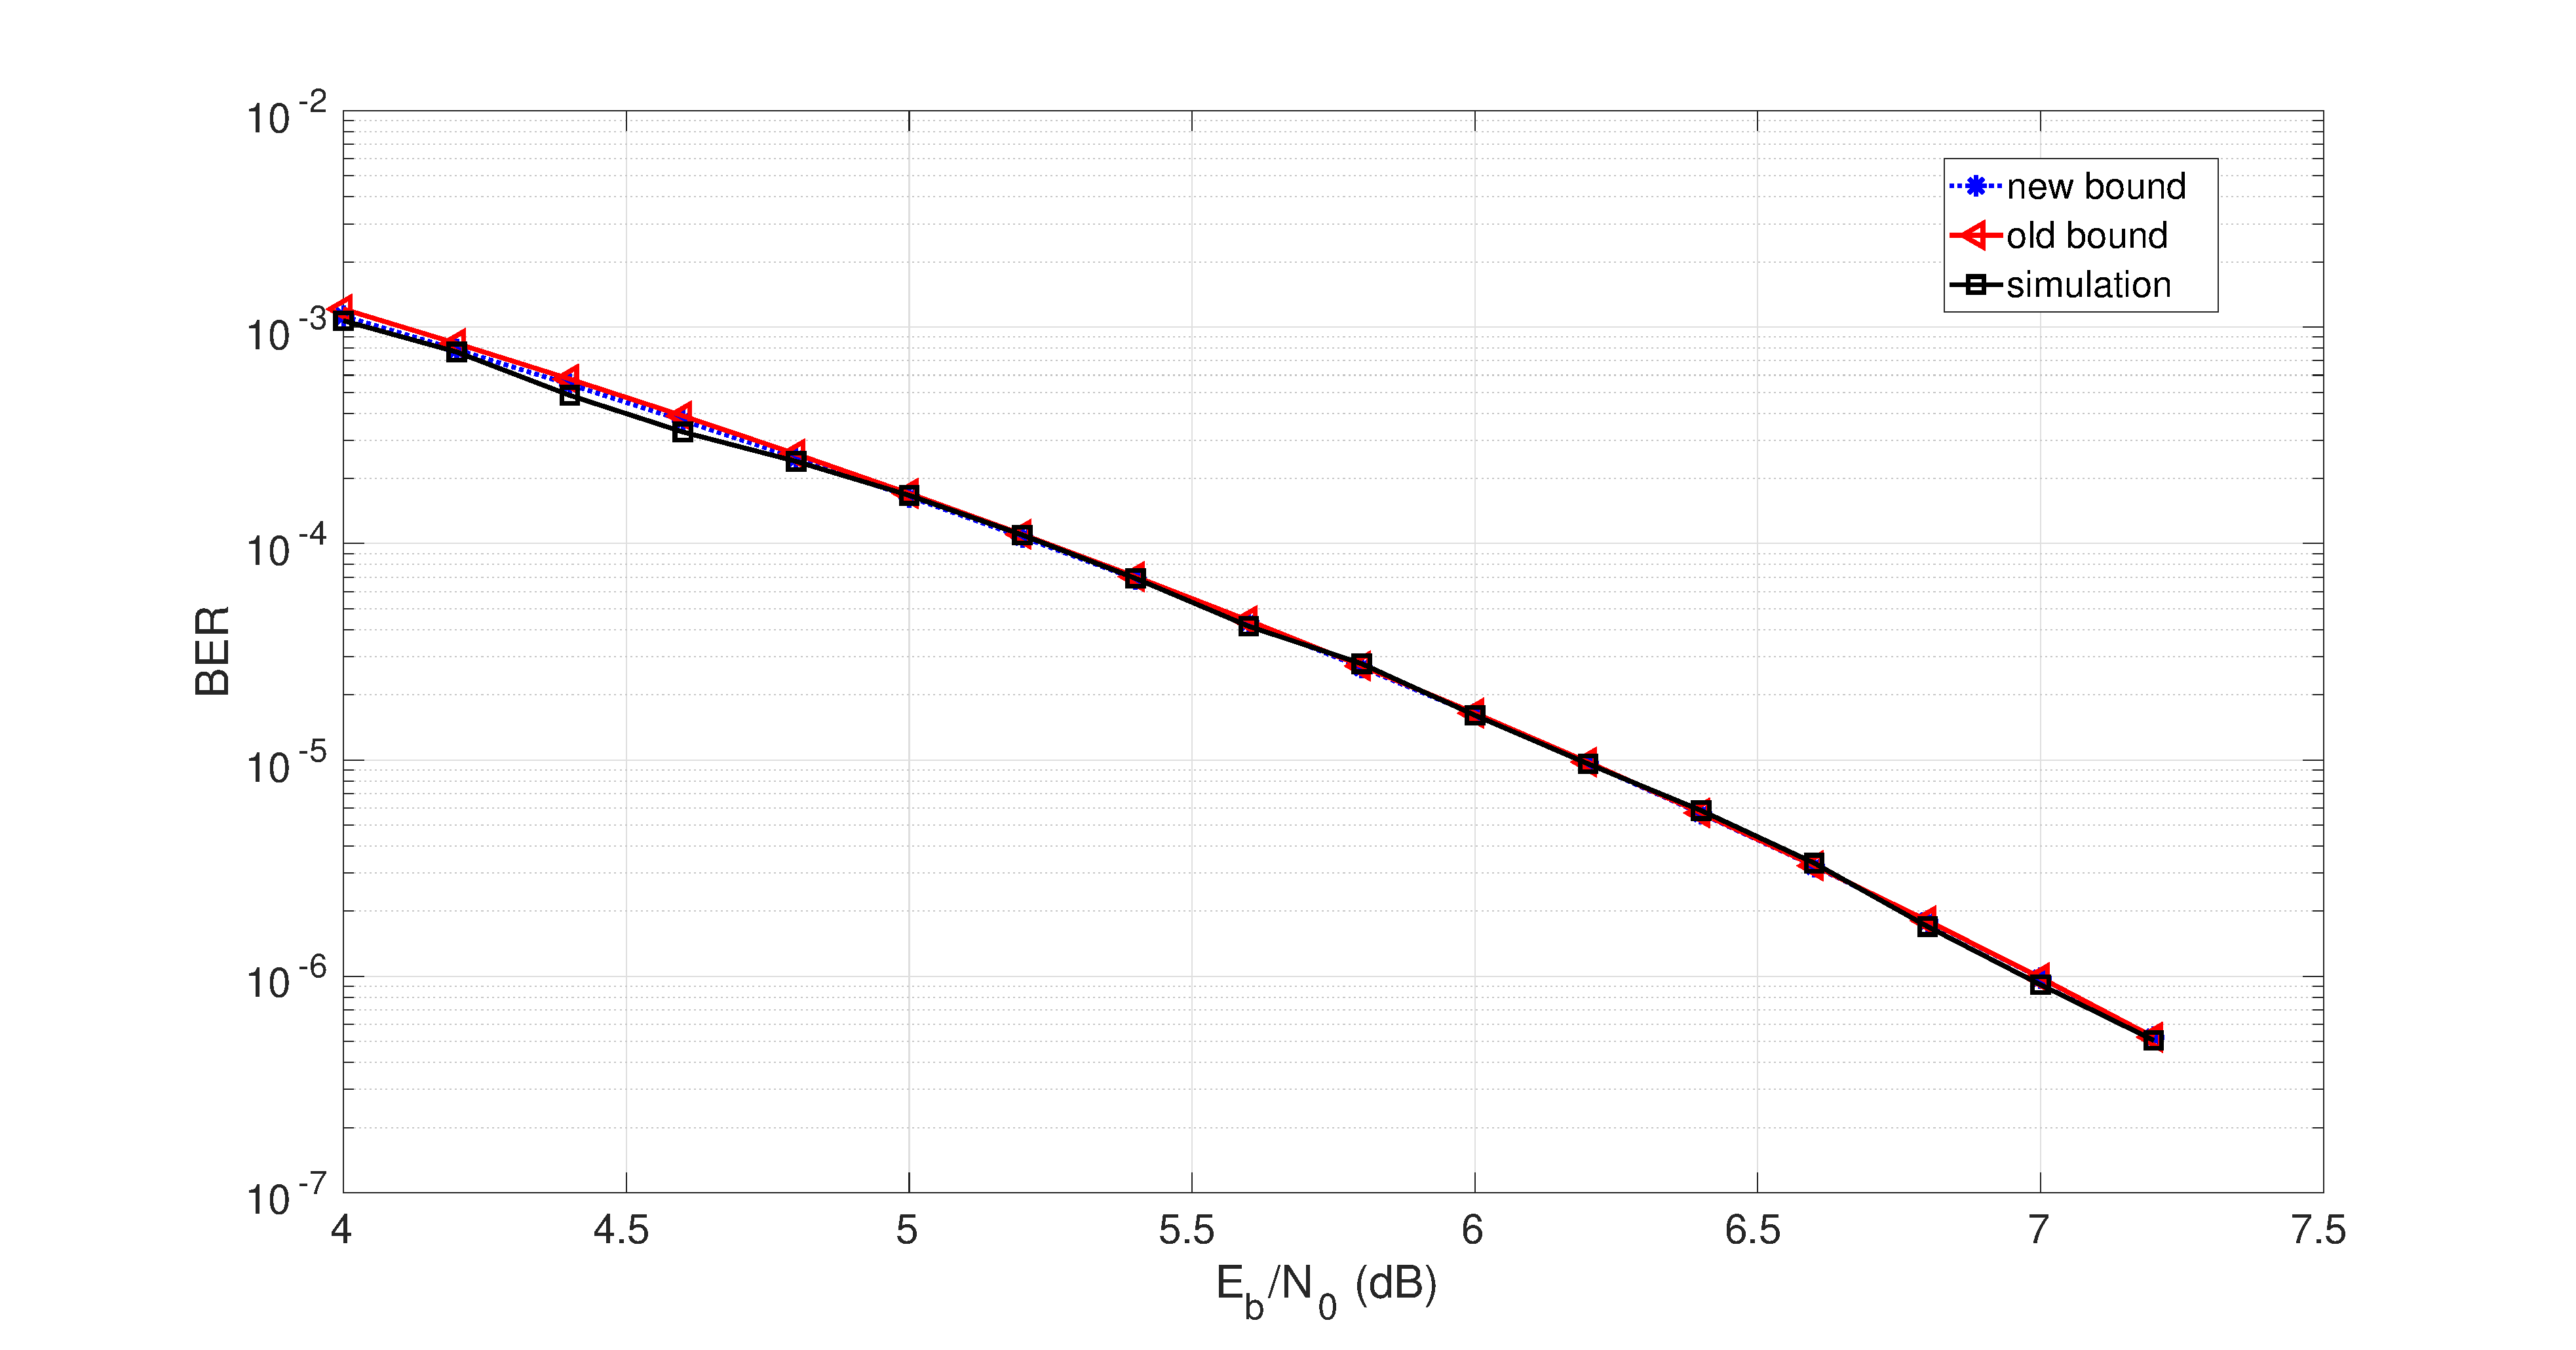
\includegraphics[width=0.5\textwidth]{./Images/RSC_5_7_lower_weights.eps}
		\captionof{figure}{Old Bound vs New Bound vs Simulation for 5/7 RSC Code}
		\label{simFig1}
		\end{figure}
		
Fig. \ref{simFig1} shows the simulation results for the $5/7$ RSC code as well as the lower bounds obtained using the transfer function as well as our novel method. The feedforward connection has the polynomial representation $1+x^2$ and can be factorized into the irreducible polynomial $1+x$. From Example \ref{ex-3}, we observe that whiles there exists weight-2 PCs, there  are no weight-3 PCs for $1+x^2$
The feedback connection has the polynomial representation $1+x+x^2$, which is an irreducuble polynomial and from Example \ref{ex-1}, we can confirm that there exists weight-2 SCs as well as weight-3 SCs. In Fig. \ref{simFig1}, we observe that there is some difference between the new (novel method) bound and the old (transfer function) bound, but they tend to converge as $E_b/N_0$ increases. This suggests that the approximation $ \bigcup_{d = d_{\text{min}}}^{d_{\text{max}}} \cA'_c(d) $ used in our novel method is sufficient for the $5/7$ RSC code.

%We observe that for both Fig. \ref{simFig1} and Fig. \ref{simFig2}, there is some difference between the new (novel method) bound and the old (transfer function) bound, but they tend to converge as $E_b/N_0$ increases. This suggests that the approximation used with our novel method is sufficient for these RSC codes.

%codewords generated considering $b(x),~w_H(b(x))>3$ as well as codewords which have a parity-check sequence $h(x),~w_H(h(x))>3$ do not have much effect on the BER of the code as $E_b/N_0$ increases.

%The gap that is observed in the low $E_b/N_0$ regions is attributed to omitting codewords generated by the RTZ inputs of weight $w_H(\bb)=4$ as well as codewords with parity-check sequences $w_H(\bh)=4$ in our calculation of the new bound. 

%Fig. \ref{simFig4} and Fig. \ref{simFig5} are similar to  Fig. \ref{simFig1} and Fig. \ref{simFig2}, with the only difference being that codewords generated by the RTZ inputs of weight $w_H(\bb)=4$ as well as codewords with parity-check sequences $w_H(\bh)=4$ have been added in our calculation of the new bound. The new and old bounds match up and the accuracy of our bound is greatly improved.The simulation results also agree with the bounds as they also converge with the bounds.

\begin{table}[htbp]
 \caption{Partial Codeword Component Pattern Distance Spectrum for the $37/21$ RSC code, $d_{\text{free}}=6$}
\centering
 \begin{tabularx}{0.75\textwidth}{Xlll} 
 \hline
 $w_H(c(x))$&$a(x)$ & $b(x)$ & $h(x)$ \\ [0.5ex] 
 \hline\hline
6&$1+x$ & $1+x+x^{4}+x^5$ & $1+x^5$\\
\hline\hline
7&$1$ & $1+x^4$ & $1+x+x^2+x^3+x^4$\\
\hline\hline
8&$1+x+x^5+x^6$ & $1+x+x^4+x^6+x^9+x^{10}$ & $1+x^{10}$\\
\hline
%$1+x+x^4+x^5$ & $1+x+x^8+x^9$ & $1+x^4+x^5+x^9$\\
%\hline
%$1+x^2$ & $1+x^2+x^4+x^6$ & $1+x+x^5+x^6$\\
%\hline
%$1+x+x^5$ & $1+x+x^4+x^9$ & $1+x^6+x^7+x^8+x^9$\\
%\hline
%$1+x+x^4$ & $1+x+x^5+x^8$ & $1+x^4+x^6+x^7+x^8$\\
%\hline
%$1+x^2+x^4$ & $1+x^2+x^6+x^8$ & $1+x+x^4+x^7+x^8$\\
%\hline
%$1+x^3+x^4$& $1+x^3+x^7+x^8$ & $1+x+x^2+x^4+x^8$\\
%\hline
%$1+x^4+x^5$ & $1+x^5+x^8+x^9$ & $1+x+x^2+x^3+x^9$\\
 \end{tabularx}
 
 \label{novelTab14}
\end{table}

\begin{figure}[htbp]
\centering
		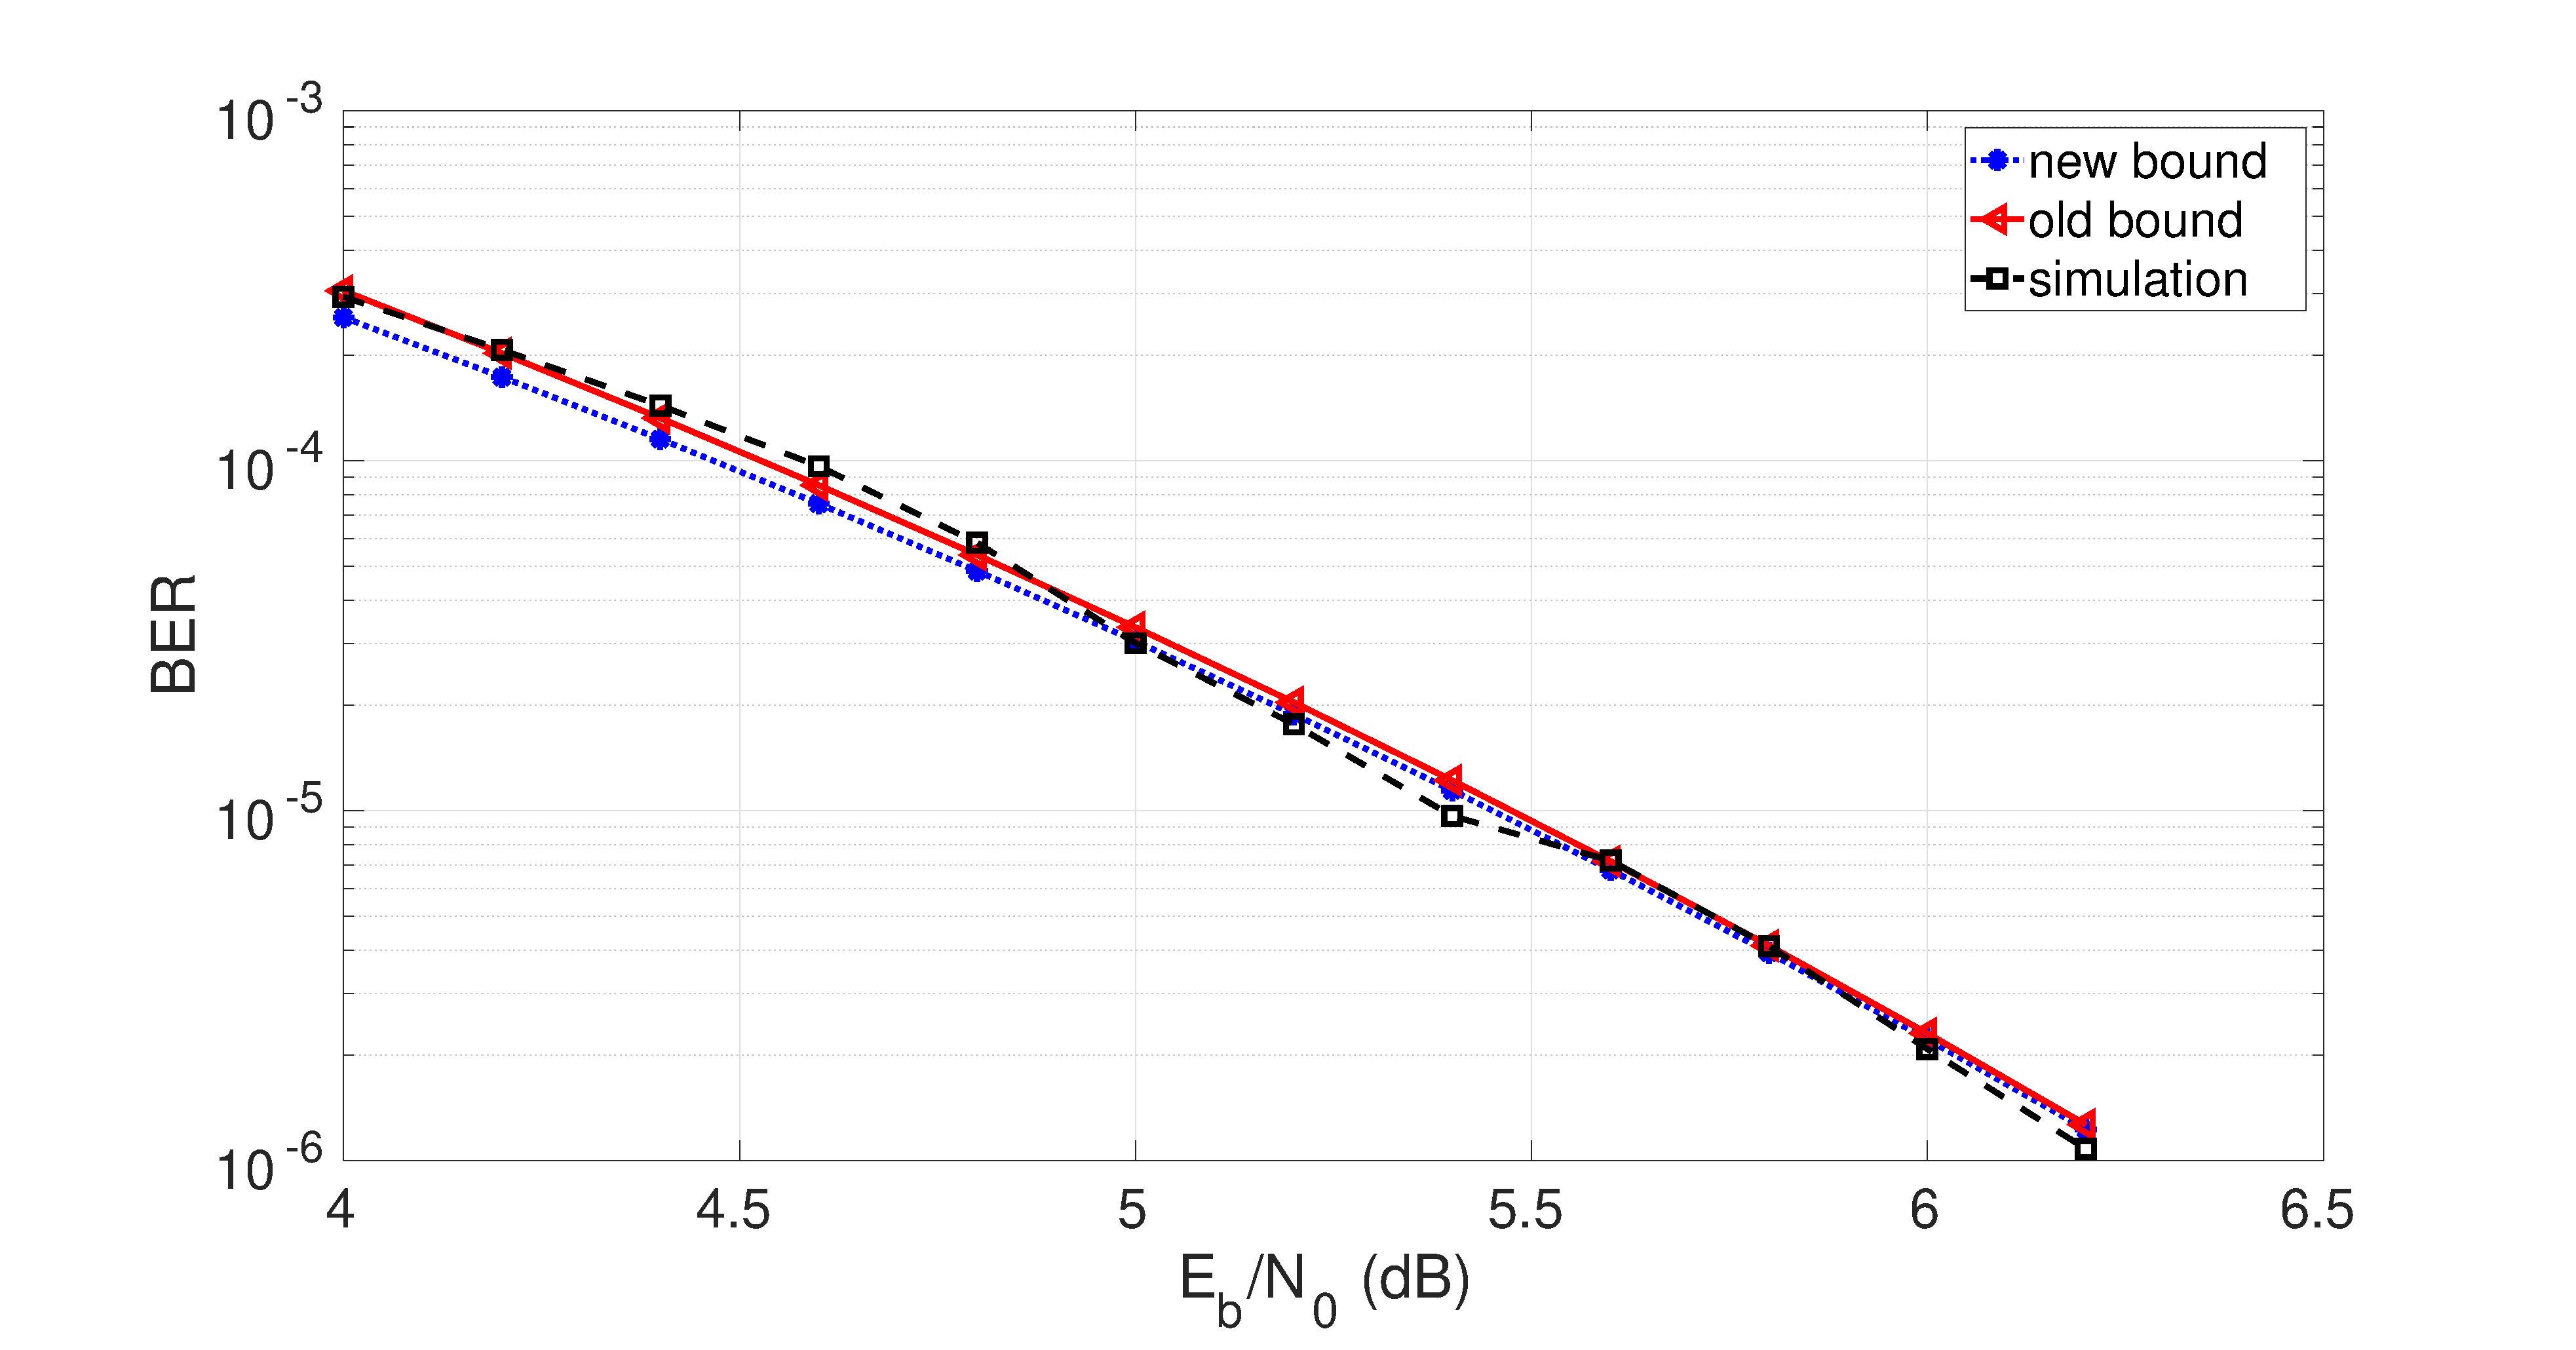
\includegraphics[width=0.5\textwidth]{./Images/RSC_37_21_lower_weights.eps}
		\caption{Old Bound vs New Bound vs Simulation for 37/21 RSC Code}
		\label{simFig2}
		\end{figure}
Fig. \ref{simFig2} shows the simulation results for the $37/21$ RSC code as well as the lower bounds obtained using the transfer function as well as our novel method. The feedforward connection has the polynomial representation $1+x+x^2+x^3+x^4$, which is an irreducible polynomial. From Example \ref{ex-2}, we confirm that whiles weight-2 PCs exist, there are no wight-3 PCs. The feedback connection has the polynomial representation $1+x^4$, and from Example \ref{ex-3}, we can deduce that weight-2 SCs exist, but there are no weight-3 SCs. In Fig. \ref{simFig2}, we observe that there is some difference between the new (novel method) bound and the old (transfer function) bound, but they tend to converge as $E_b/N_0$ increases. This suggests that the approximation $ \bigcup_{d = d_{\text{min}}}^{d_{\text{max}}} \cA'_c(d) $ used in our novel method is also sufficient for the $37/21$ RSC code.
%In \ref{simFig3}, we observe that the old bounds and simulation results converge as the Eb/No value increases. However, there is a very distinct gap between the new bound and the old bound. Moreover, the bounds do not converge as the Eb/No increases. This suggests that the approximation used in our novel method is insufficient for this RSC code and considering  $w_H(h(x)),~w_H(b(x))=4$ might yield a more accurate bound.

\begin{table}[htbp]
 \caption{Partial Codeword Component Pattern Distance Spectrum for the $23/35$ RSC code, $d_{\text{free}}=7$}
\centering
\begin{tabularx}{0.75\textwidth}{lXlX} 
 \hline
$w_H(c(x))$ & $a(x)$ & $b(x)$ & $h(x)$ \\ [0.5ex] 
 \hline\hline
7&$1+x^2+x^3$ & $1+x^7$ & $1+x+x^2+x^6+x^7$\\
\hline
&$1$ & $1+x^2+x^3+x^4$ & $1+x+x^{4}$\\
\hline \hline
8&$1+x+x^2+x^3+x^5$ & $1+x^3+x^4+x^8+x^9$ & $1+x^7+x^9$\\
\hline\hline
9&$1+x+x^2+x^3+x^5+x^7+x^8$ & $1+x+x^3+x^4+x^7+x^{12}$ & $1+x^{11}+x^{12}$\\
\hline\hline
10&$1+x^2+x^3+x^7+x^9+x^{10}$ & $1+x^{14}$ & $1+x+x^2+x^6+x^8+x^9+x^{13}+x^{14}$\\
\hline
 \end{tabularx}
 
 \label{novelTab15}
\end{table}

\begin{figure}[htbp]
\centering
		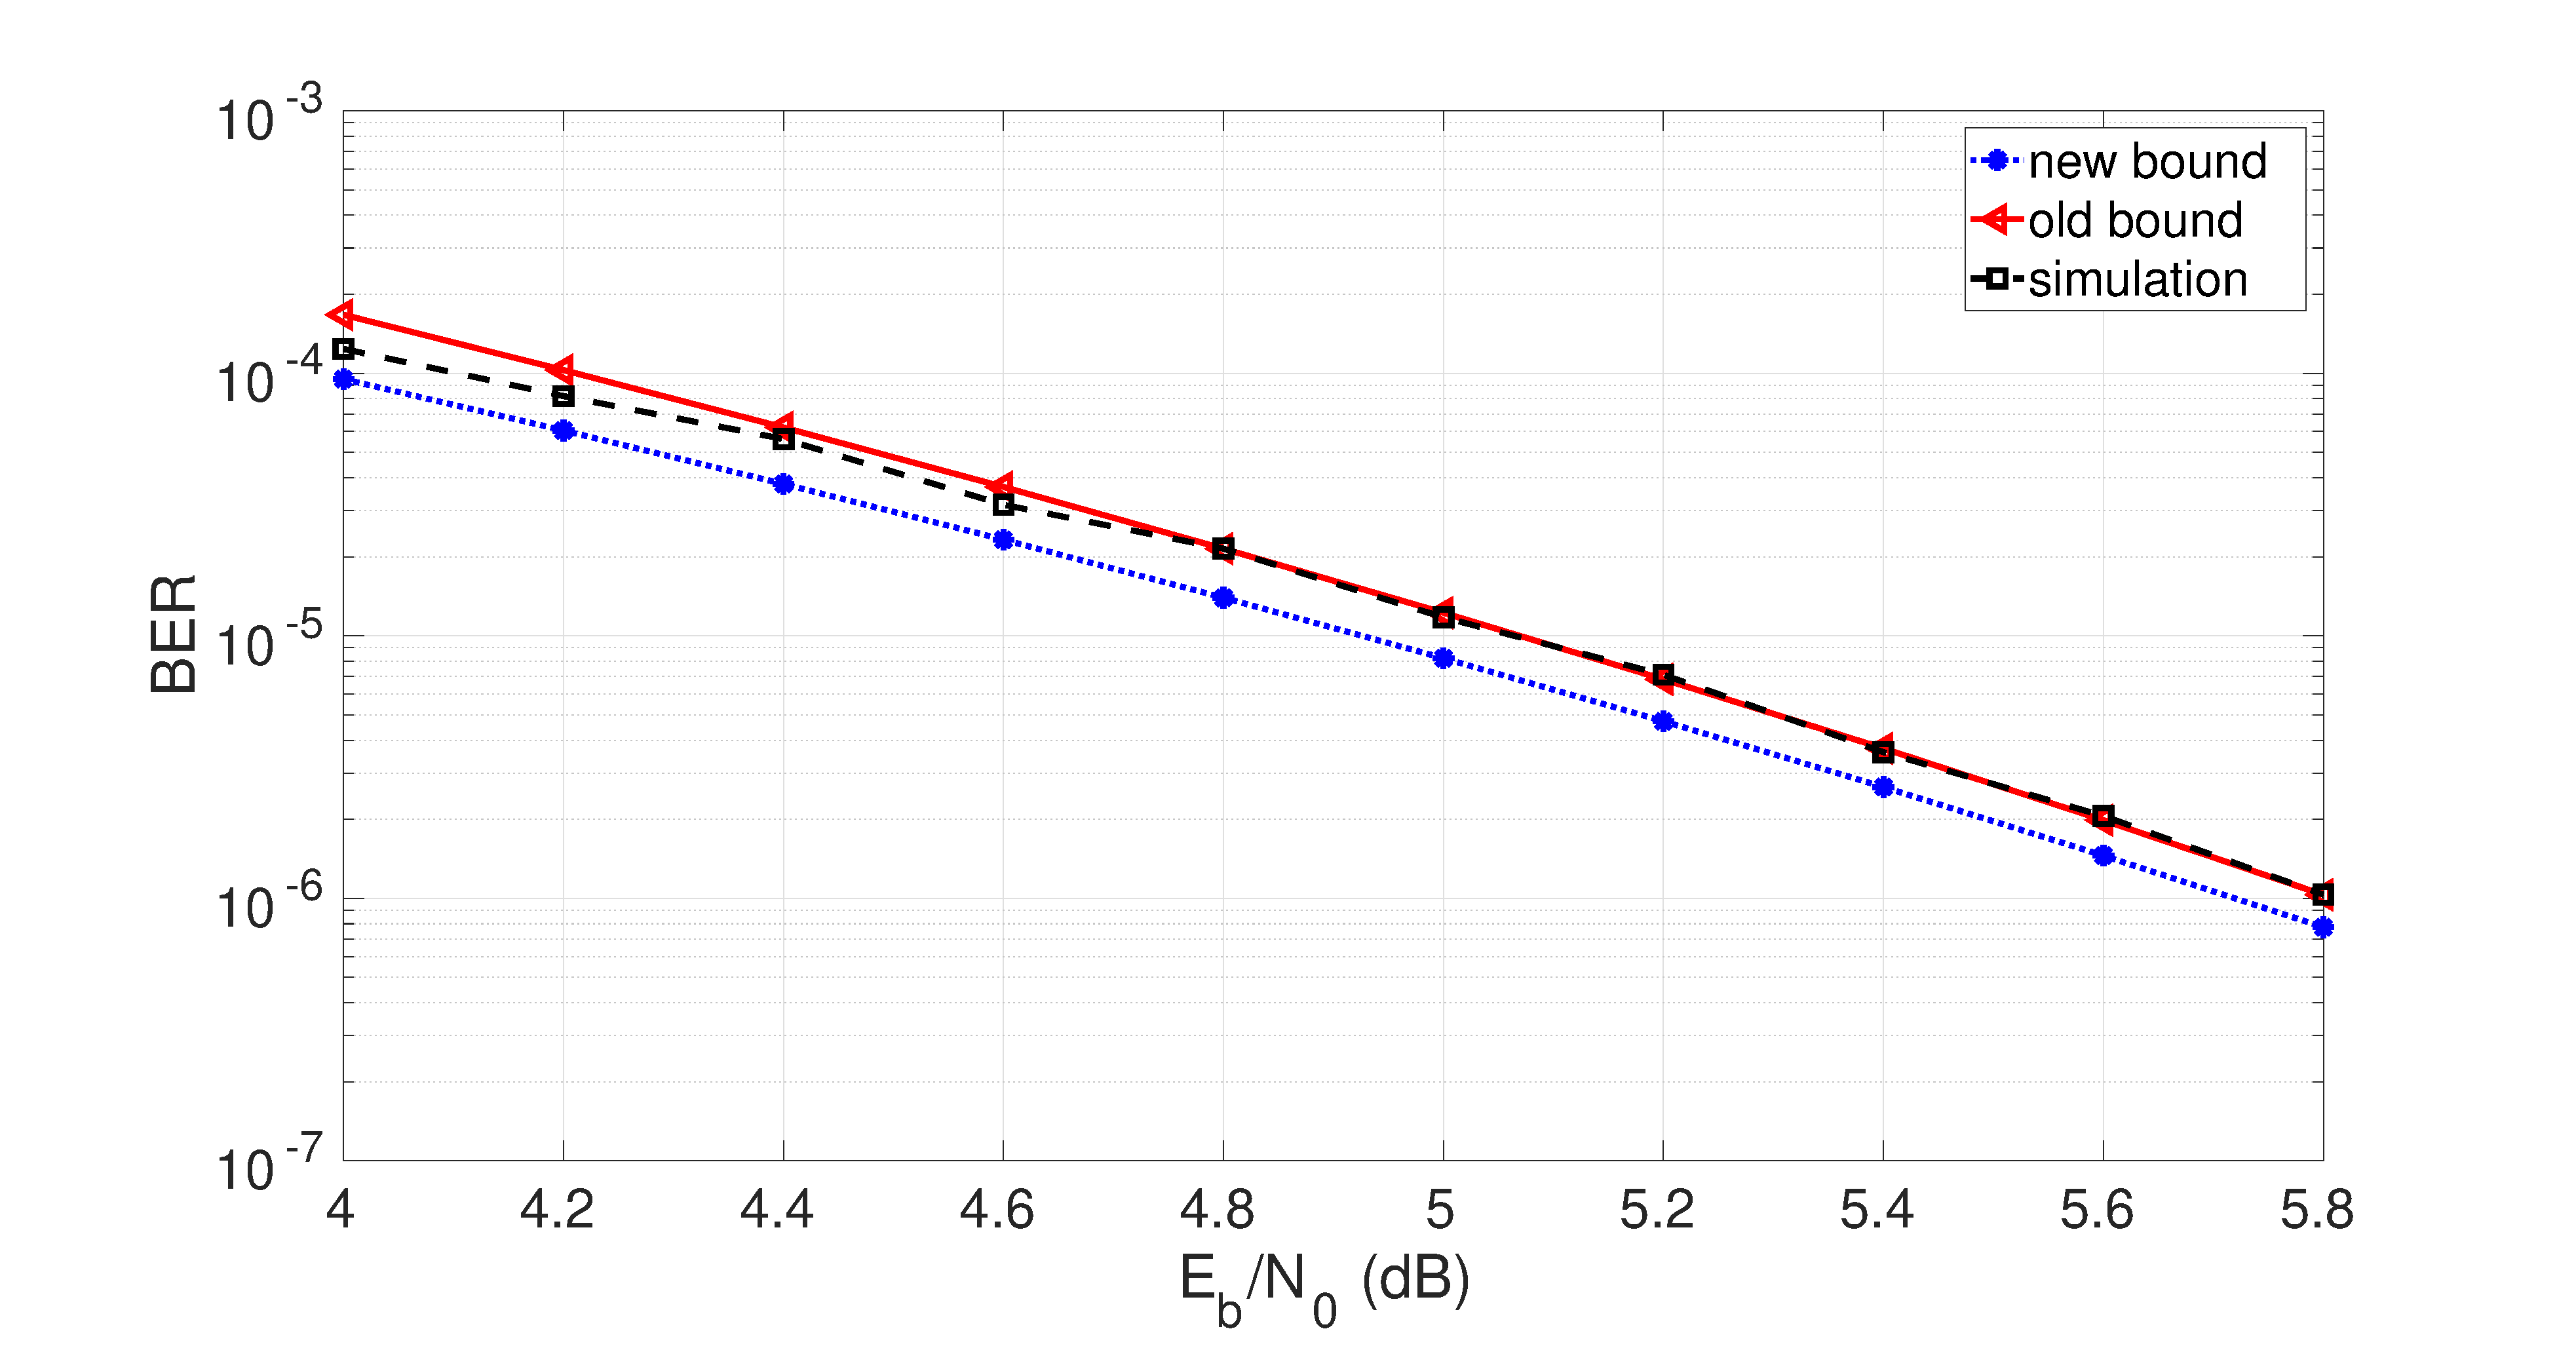
\includegraphics[width=0.5\textwidth]{./Images/RSC_23_35_lower_weights.eps}
		\caption{Old Bound vs New Bound vs Simulation for 23/35 RSC Code}
		\label{simFig3}
		\end{figure}
Fig. \ref{simFig3} shows the simulation results for the $23/35$ RSC code as well as the lower bounds obtained using the transfer function as well as our novel method. The feedforward connection has the polynomial representation $1+x+x^4$, which is similar in characteristic to the polynomial in Example \ref{ex-1}. It can easily be confirmed that there exists weight-2 and weight-3 PCs. For the weight-2 PCs, the general form for $a(x)$ is
\begin{equation*}
a(x)=\sum_{\ell=0}^{L-1} x^{15\ell}(1+x+x^{2}+x^3+x^5+x^7+x^8+x^{11})
\end{equation*}
and since it yields codewords such that $w_H(c(x))>d_{\text{max}}$, there are not included in our approximation of the lower bound, as can be observed from Table \ref{novelTab14}. The feedback connection has the polynomial representation $1+x^2+x^3+x^4$, which can be factorized into $2$ irreducible polynomials and it can easily be confirmed that there exists no weight-3 SCs, since $1+x$ is a factor. In Fig. \ref{simFig3}, we observe that the old (transfer function) bounds and simulation results converge as the $E_b/N_0$ value increases. However, there is some difference between the new (novel method) bound and the old (transfer function) bound, even as $E_b/N_0$ increases. This suggests that the approximation used in our novel method is insufficient for this $23/35$ RSC code and considering  $w_H(h(x)),~w_H(b(x))=4$ might yield a more accurate bound.


%\begin{figure}[h!]
%\centering
%		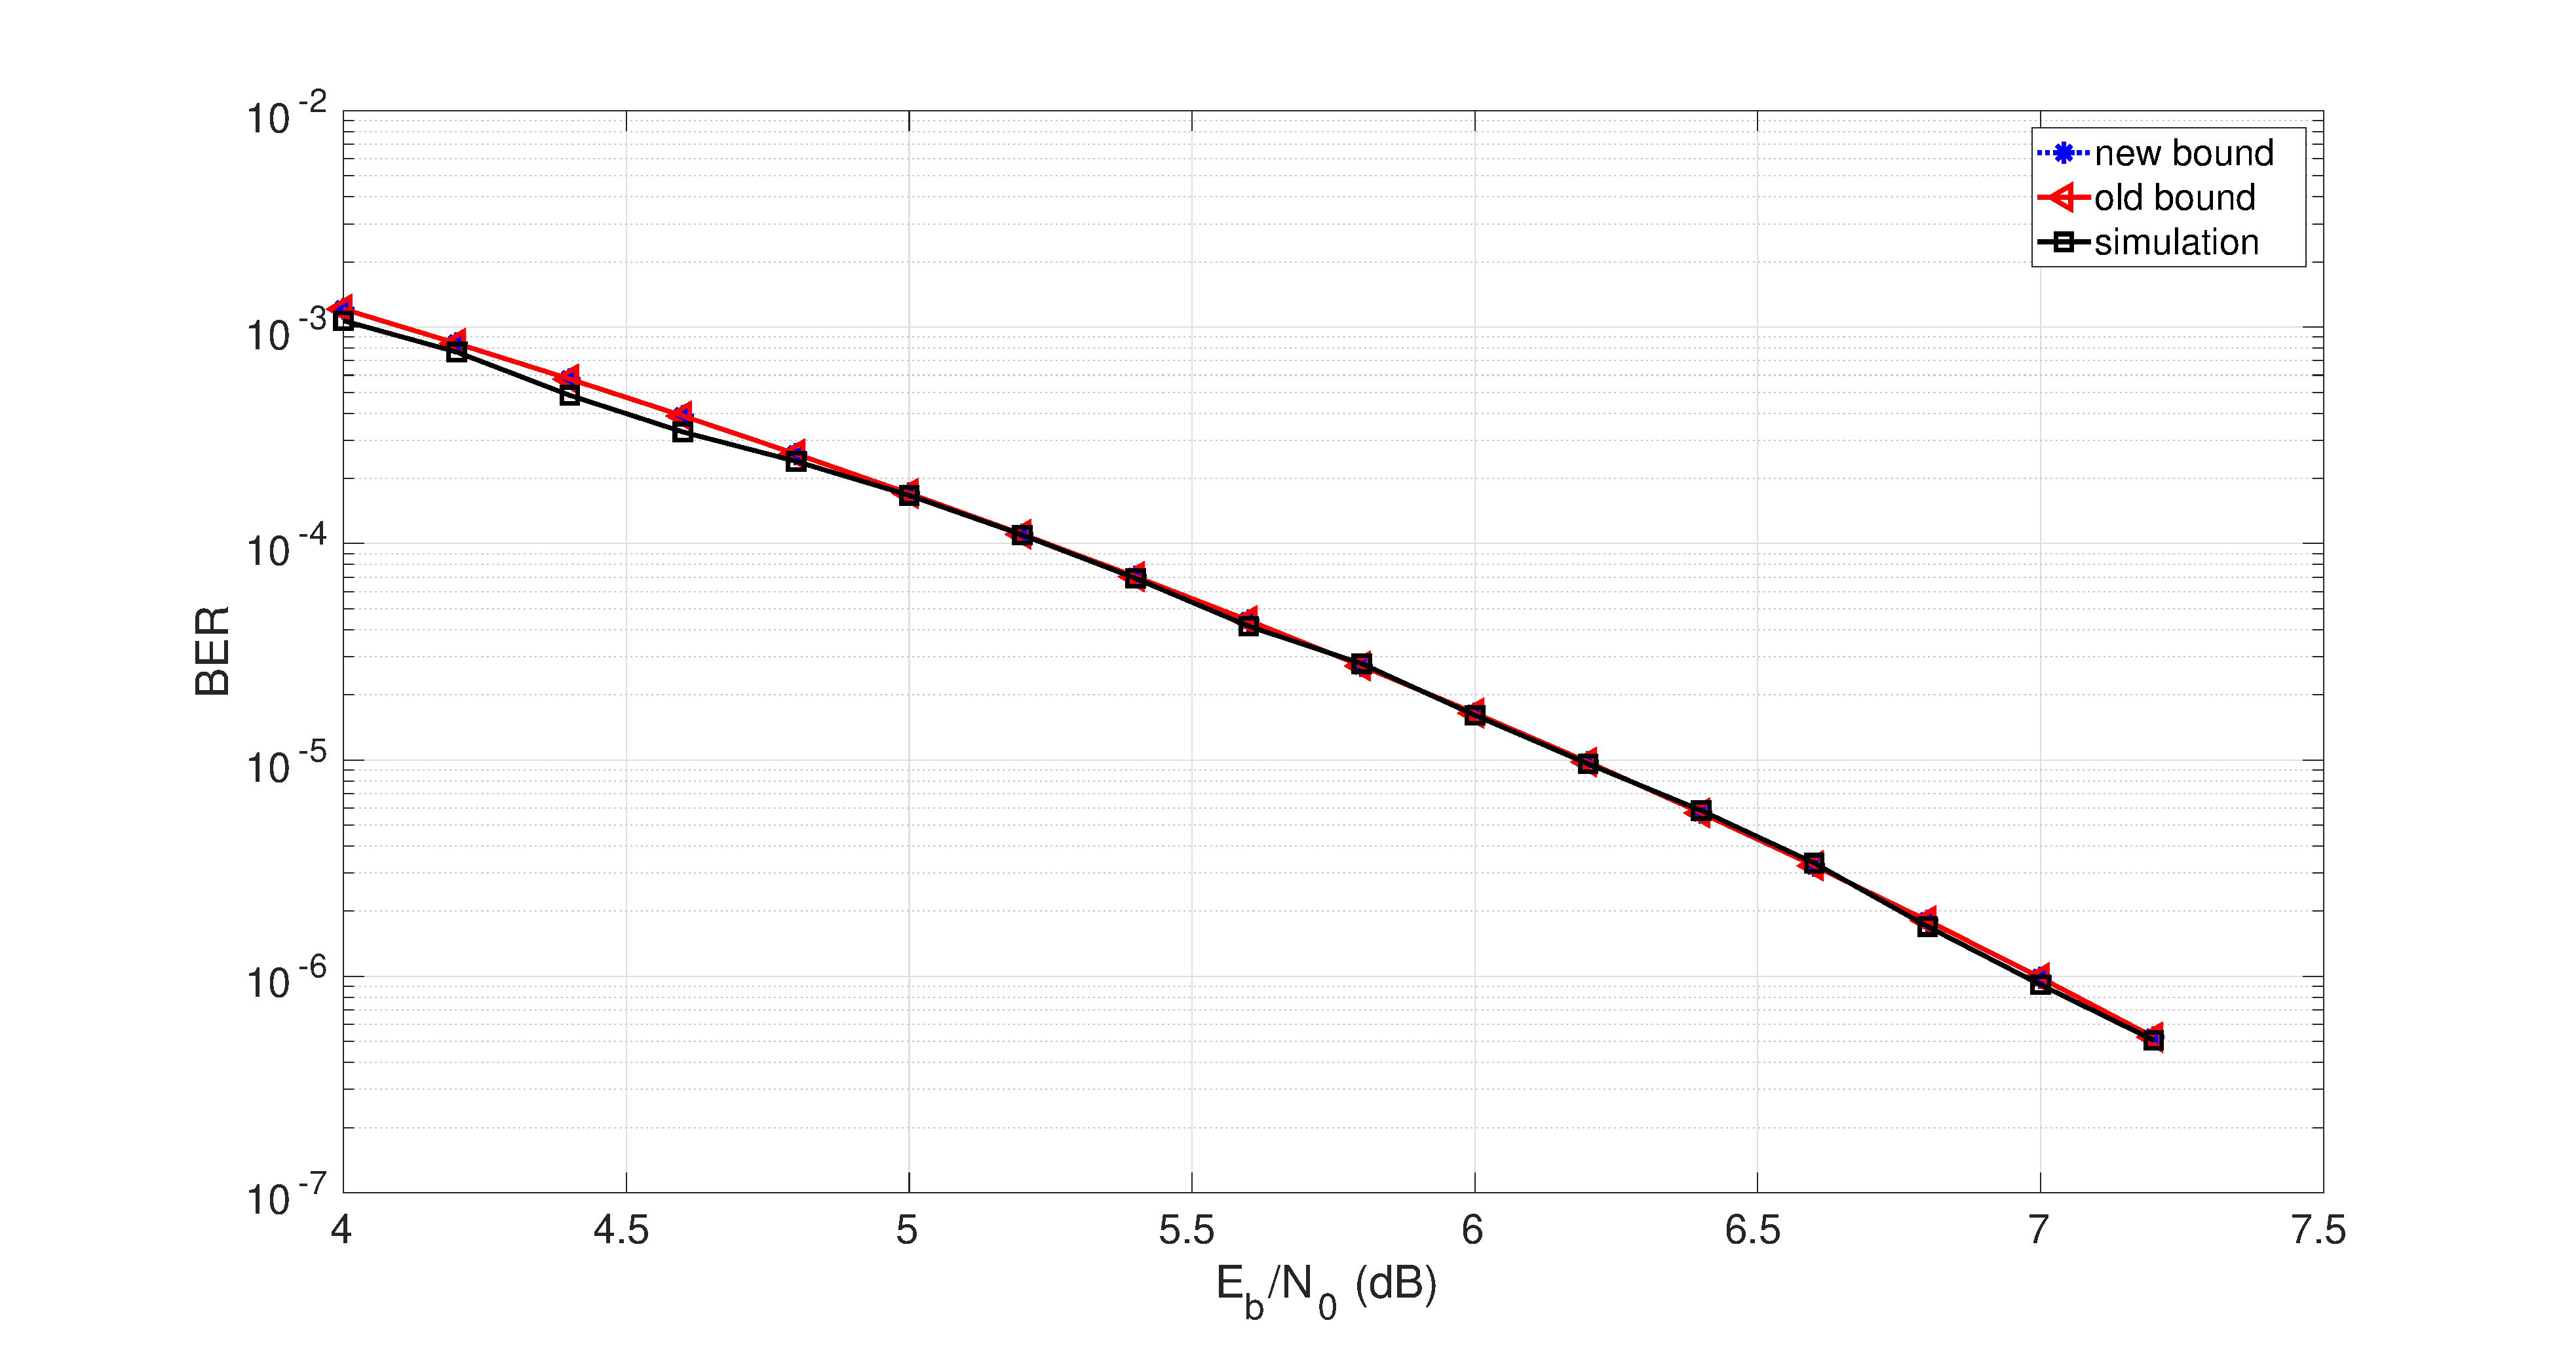
\includegraphics[width=0.8\textwidth]{./Images/RSC_5_7_higher_weights.eps}
%		\caption{Old Bound vs New Bound vs Simulation for 5/7 RSC Code, with higher weights }
%		\label{simFig4}
%		\end{figure}
		
		
%		\begin{figure}[h!]
%\centering
	%	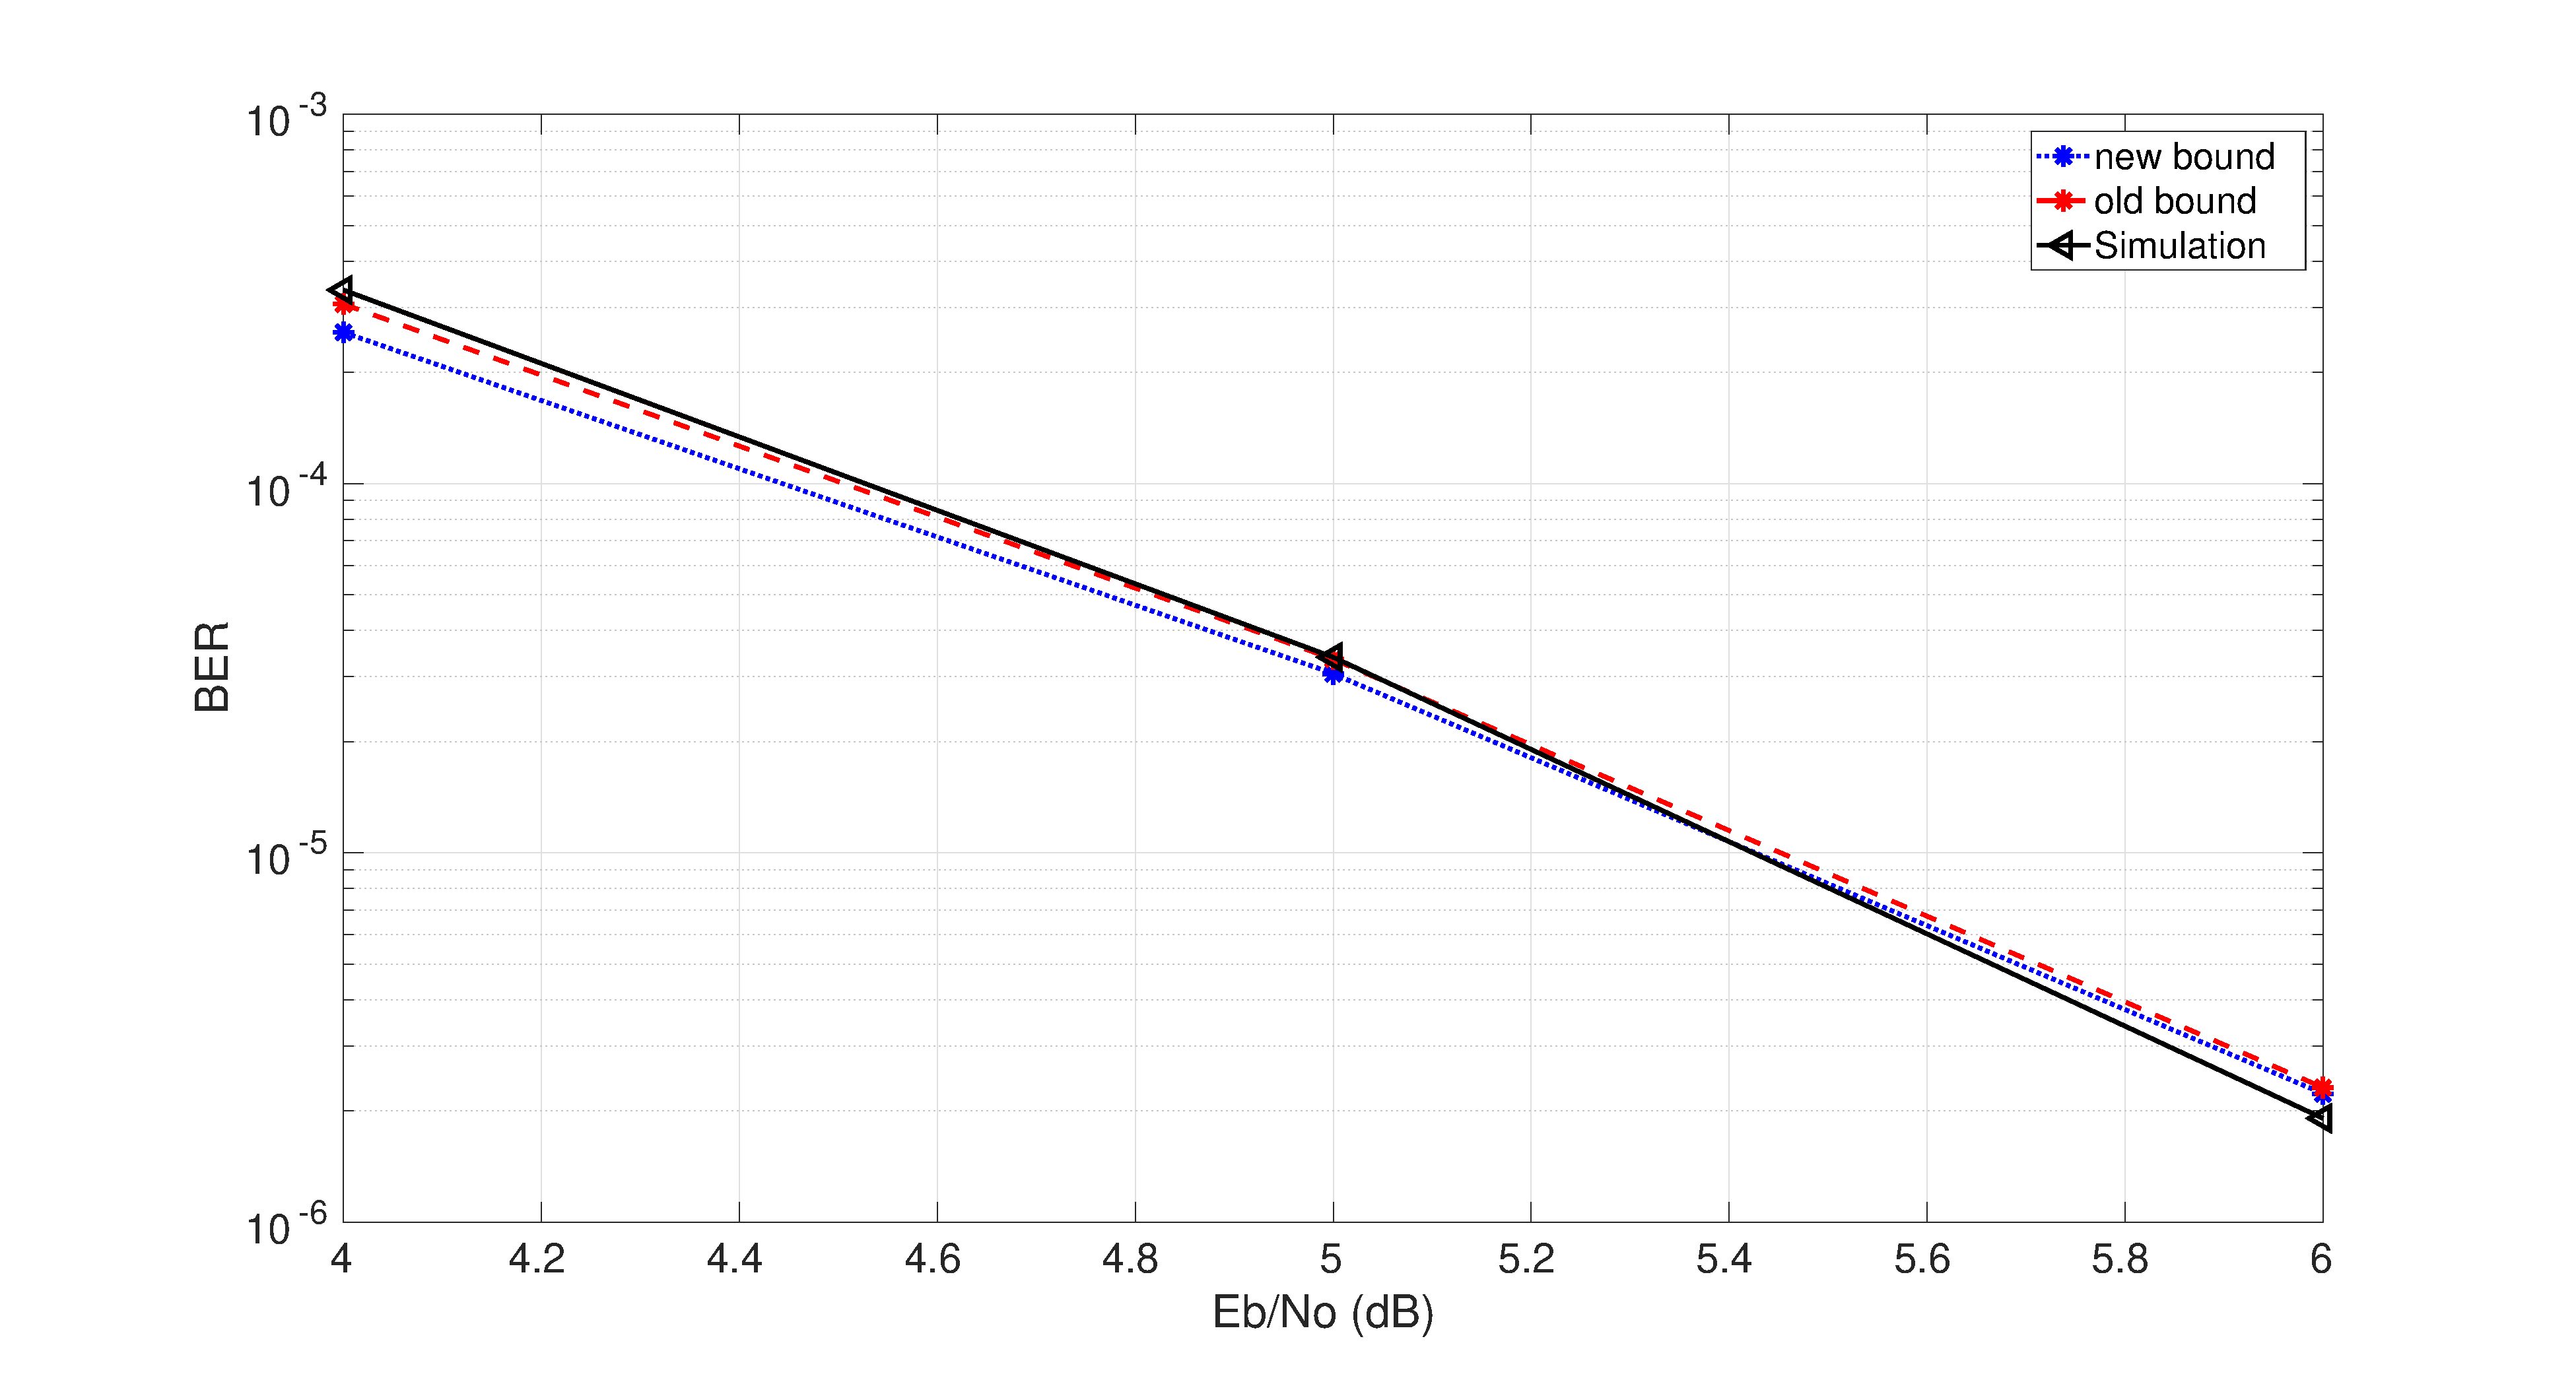
\includegraphics[width=0.5\textwidth]{./Images/RSC_37_21_v2.eps}
		%\caption{Old Bound vs New Bound vs Simulation for 37/21 RSC Code, with higher weights}
		%\label{simFig5}
		%\end{figure}


